\chapter{Motivation}


\begin{figure}[ht]
  \centering
  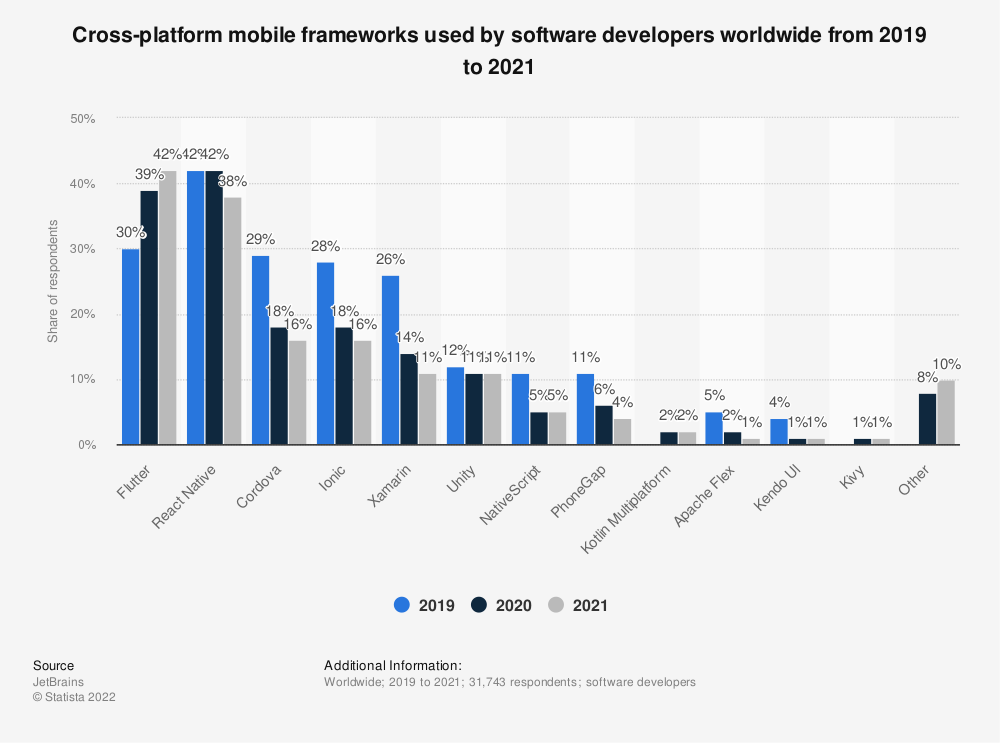
\includegraphics[height=7cm,keepaspectratio]{images/cross-platform-mobile-frameworks.png} 
  \caption{Cross-Plattform-Frameworks 2019-2021}
  \label{fig:statista_cross_plattform}
\end{figure}

Abbildung \ref{fig:statista_cross_plattform} zeigt Statistik von JetBrains die Verteilung von verschiedenen Sprachen zeigt: Abbildungsverzeichnis hinzufügen dafür

Die Entwicklung im Bereich der mobilen Anwendungsentwicklung ist in den letzten Jahren sehr hoch. Nicht nur das immer mehr Technologien und Frameworks in Richtung Hybride Appentwicklung entwickelt werden. Es werden auch immer mehr Erweiterungen für bestehende Technologien geschrieben, die eine möglichst effiziente mobile App ermöglichen sollen. Aber auch die nativen Apps ändern sich stetig und die dahinter stehenden Programmiersprachen bekommen stetig neue Änderungen und werden weiterentwickelt.

Wenn man nun eine eigene Applikation schreiben will, steht man erstmal vor der Frage wie und wo man anfängt.
Fragen nach der richtigen Programmiersprache bzw. dem richtigen Framework kommen dann auf.

Langezeit gab es hier sehr konkrete Antworten. Da die meisten leute vlt. nur einen Heimcomputer besaßen, entwickelte man meist nur Computeranwendungen oder eben Webapplikationen, die jeder von überall aus aufrufen konnte, ohne die Applikation auf seinem eigenen Computer installieren zu müssen.

Mit der Ära der Smartphones jedoch änderte sich das etwas, denn auch hier kann man natürlich Webapplikationen nutzen, jedoch sind diese oft nicht angepasst gewesen.

Daraus entstand eine Zeit wo mobile Applikationen speziell für das eigene Smartphone entwickelt wurden. Es gab auch einige neue Ansätze und Funktionalitäten, die man so nutzen konnte, die davor nicht nutzbar waren. Hier wurden oft Applikationen mit Swift, der Programmiersprache für iOS und Java bzw. mittlerweile Kotlin für Android Applikationen. Hier entstanden also sogar eigene Programmiersprachen für die jeweiligen Plattformen zur sogennanten nativen Entwicklung.

Wenn man jedoch nun auf mehreren Plattformen seine Applikationen veröffentlichen wollte, so musste man zwei eigene Applikationen in zwei unterschiedlichen Programmiersprachen schreiben. 

Daraus entstand der Wille dass doch zu vereinigen und 
sogennante Multi-Plattform-Applikationen oder auch Cross-Plattform-Applikationen zu entwickeln.
Und hier fing das Problem an. Da dies eine frei Entwickelte Sache war, wo zunächst keiner der großen Plattformanbieter dahinter stand, entstanden viele kleine und auch manchmal größere Frameworks die dieses Problem lösen sollte.

In dieser Zeit gab es auch immer wieder Ansätze großer Firmen, ihre Apps in hybride Apps zu ändern, jedoch tauchen auch immer wieder Berichte darüber auf, dass solche Schritte nach einer anfänglichen Testzeit wieder aufgegeben wurden. So hat etwa Airbnb bereits 2016 mit sogenannten React Native versucht ihre Apps auf eine gemeinsame Codebasis zu bauen. Sie haben das auch einige Zeit probiert, haben dann allerdings 2018 eine Reihe von Blog Einträgen veröffentlicht, in der sie erklären, warum sie React Native damals dann aufgegeben haben und dabei erklärt, dass sie sich deshalb weiter darauf konzentrieren würden, die nativen Apps zu verbessern. 
\TODO{Hier mehr zu den Gründen schreiben warum aufgegeben}
Durch Beispiele wie dieses, waren App-Entwickler lange Zeit skeptisch gegenüber derartigen Lösungen, da dies auch immer mit großen Änderungen und hohen Investments verbunden waren.
Jedoch gab und gibt es mittlerweile immer mehr Ansätze die es scheinbar schaffen diese Hürden zu überwinden.
\cite{MaiThiNguyenKim.}

Durch aber die eben geschilderte Entwicklung und Berichte, ist die Meinung die man hierzu lesen kann immer sehr unterschiedlich und stark von eigenen Erfahrungen abhängig. 
Deswegen soll in dieser Arbeit drei unterschiedliche Ansätze mit beispielhaften Frameworks und Programmiersprachen betrachtet werden um am Ende vlt eine bessere Einschätzung geben zu können, wie eine solche Entscheidung ausfallen könnte und Gründe für und gegen bestimmte Ansätze geben.
\TODO{umschreiben}
Auch als Appentwickler nehmen durch immer neue Technologien die entwickelt werden und auch erfolgreich teilweise eingesetzt werden, die Anfragen zu, die eine Entwicklung mit Hilfe von Flutter oder ähnlichen Wünschen. Dennoch ist es immer noch ein Verfahren, das weiter untersucht werden muss und noch nicht überall selbst verständlich benutzt unnd entwickelt werden kann.

Daher ist der Fokus dieser Arbeit einmal an einigen konkreten Beispielen zu untersuchen, wie der aktuelle Stand der Technologie hier ist und zu erforschen, welche Einschränkungen die Frameworks besitzen um hier auch eine gewisse Bewertung zu Benutzbarkeit als Applagentur zu untersuchen.

------
Schon genauere Erklärung:
Wenn man die Idee zu einer App hat, gibt es die große Frage, wie man nun anfängt und welche Programmiersprache / Framework man wählt. Hierfür gibt es ganz verschiedene Ansätze.  

Jedoch noch grundlegender ist die Frage nach der Plattform. Es gab lange Zeiten in der Applikationsentwicklung, dass nur eine Webversion veröffentlicht wurde. Mittlerweile nutzen jedoch viele Menschen nur noch ihr Smartphone und wollen dementsprechend auch nur mit mobilen Versionen auskommen. Man kann natürlich auch im Web veröffentlichte Applikationen auf dem Handy nutzen, jedoch gibt es hier zwei Sachen, die dazu führen können, dass man eine eigenständige App entwickelt.
1. Eine auf mobile angepasste UI. - Auch wenn es heutzutage in fast jedem Framework und vor allem in den gängigen UI-Frameworks verschiedene Ansätze gibt, die eine recht nutzerfreundliche Version für mobilgeräte anbieten, oder manchmal auch sogar komplett eigenständige Oberflächen für mobil angezeigt werden, so kann es doch sinvoll sein, nochmal extra angepasste UI in Form einer Applikation nativ für die Geräte zu entwickeln. Dadurch kann man gezielt Oberflächen für die Plattformen bauen und dabei auf Plattform eigene Design Unterstützungen zugreifen. Die eine Bedienung um einiges besser machen.
2. Nutzung von Hardwarefunktionalität. -  Ein noch viel wichtigerer Punkt ist es, Funktionalität die mobile Endgeräte anbieten, zu nutzen, die etwa auf einem PC nicht nutzbar sind. Dazu zählen unter anderem GPS-Nutzung, Kamerafunktionalitäten, Bluetooth-Verbindungen,.... Diese können zwar mnanchmal auch durch einen PC geboten sein, jedoch ist es hier nicht gegeben, während man bei einem Smartphone sicher davon ausgehen kann, dass die Kamera genutzt werden kann. So können einige Geschäftsprozesse der Applikationen vereinfacht oder umgestaltet werden, so dass eine Nutzung der Applikation für den Nutzer einfacher wird, bzw. es können auch neue Funktionalitäten daraus ergeben, die es eventuell davor nicht gab.

Wenn nun die Entscheidung getroffen wurde, dass man eine mobile Applikation entwickeln will, so gibt es nun verschiedene Ansätze bzw. Frameworks, die zur Verfügung stehen. Dabei gibt es viele verschiedene Frameworks die auf den ersten Blick das selbe tun, aber doch recht unterschiedlich sein können und unter gewissen Ummständen sich manche besser eignen als andere. 
Eine der ersten Fragen die dabei im Raum steht. Gibt es bereits eine Webversion der Applikation.
Wenn nicht, so kann es von Anfang an spannend sein, ein Framework zu wählen, dass wie Flutter eine Cross-Plattform-Applikation erzeugt, wo auch eine Webversion mit gehostet werden kann.
Falls es bereits eine Webversion geben, so geht der Weg eher in Richtung von Nativen- bzw. Hybriden Applikationen, da meißt nur noch einzelne Teile der Applikation entwickelt werden müssen. Dies ist jedoch auch kein Grund eine Cross-Plattform-Entwicklung auszuschließen, da dadurch nur ein Code geschrieben werden muss um etwa beide vorherschenden mobilen Plattformen abzudecken: iOS und Android.

'''Hier könnte man so ein Art Diagramm machen mit Fragen und dann Entscheidungswegen. So nach dem Motto finde dein Framework zur entwicklung einer mobilen Applikation.'''



